\documentclass{beamer}
\usepackage[T1]{fontenc}
\usepackage[utf8]{inputenc}
\usepackage{listings}
\usepackage{amssymb}
\usepackage{upgreek}
\usepackage{mathtools}
\usepackage{graphicx}
\graphicspath{ {./images/} }
\usepackage{tikz}
\usetikzlibrary{shapes.callouts,shadows, calc}

\usepackage[dvipsnames]{xcolor}
%colors for lean syntax
\definecolor{keywordcolor}{rgb}{0.7, 0.1, 0.1}   % red
\definecolor{tacticcolor}{rgb}{0.0, 0.1, 0.6}    % blue
\definecolor{commentcolor}{rgb}{0.4, 0.4, 0.4}   % grey
\definecolor{symbolcolor}{rgb}{0.0, 0.1, 0.6}    % blue
\definecolor{sortcolor}{rgb}{0.1, 0.5, 0.1}      % green
\definecolor{attributecolor}{rgb}{0.7, 0.1, 0.1} % red

\def\lstlanguagefiles{lstlean.tex}
% set default language
\lstset{language=lean}

\usetheme[compress]{Berlin}
\usecolortheme{default}

%for the code highlighting
\tikzset{note/.style={rectangle callout, rounded corners,fill=gray!20,drop shadow,font=\footnotesize}}    

\newcommand{\tikzmark}[1]{\tikz[overlay,remember picture] \node (#1) {};}    

\newcounter{image}
\setcounter{image}{1}

\makeatletter
\newenvironment{btHighlight}[1][]
{\begingroup\tikzset{bt@Highlight@par/.style={#1}}\begin{lrbox}{\@tempboxa}}
{\end{lrbox}\bt@HL@box[bt@Highlight@par]{\@tempboxa}\endgroup}

\newcommand\btHL[1][]{%
  \begin{btHighlight}[#1]\bgroup\aftergroup\bt@HL@endenv%
}
\def\bt@HL@endenv{%
  \end{btHighlight}%   
  \egroup
}
\newcommand{\bt@HL@box}[2][]{%
  \tikz[#1]{%
    \pgfpathrectangle{\pgfpoint{0pt}{0pt}}{\pgfpoint{\wd #2}{\ht #2}}%
    \pgfusepath{use as bounding box}%
    \node[anchor=base west,rounded corners, fill=green!30,outer sep=0pt,inner xsep=0.2em, inner ysep=0.1em,  #1](a\theimage){\usebox{#2}};
  }%
   %\tikzmark{a\theimage} <= can be used, but it leads to a spacing problem
   % the best approach is to name the previous node with (a\theimage)
 \stepcounter{image}
}
\makeatother

\lstset{moredelim=**[is][\btHL]{@}{@}}

\newcommand{\bA}{\mathbb{A}}
\newcommand{\bB}{\mathbb{B}}
\newcommand{\bC}{\mathbb{C}}
\newcommand{\bD}{\mathbb{D}}
\newcommand{\bE}{\mathbb{E}}
\newcommand{\bF}{\mathbb{F}}
\newcommand{\bG}{\mathbb{G}}
\newcommand{\bH}{\mathbb{H}}
\newcommand{\bI}{\mathbb{I}}
\newcommand{\bJ}{\mathbb{J}}
\newcommand{\bK}{\mathbb{K}}
\newcommand{\bL}{\mathbb{L}}
\newcommand{\bM}{\mathbb{M}}
\newcommand{\bN}{\mathbb{N}}
\newcommand{\bO}{\mathbb{O}}
\newcommand{\bP}{\mathbb{P}}
\newcommand{\bQ}{\mathbb{Q}}
\newcommand{\bR}{\mathbb{R}}
\newcommand{\bS}{\mathbb{S}}
\newcommand{\bT}{\mathbb{T}}
\newcommand{\bU}{\mathbb{U}}
\newcommand{\bV}{\mathbb{V}}
\newcommand{\bW}{\mathbb{W}}
\newcommand{\bX}{\mathbb{X}}
\newcommand{\bY}{\mathbb{Y}}
\newcommand{\bZ}{\mathbb{Z}}

\newcommand{\fC}{\mathcal{C}}
\newcommand{\fL}{\mathcal{L}}
\newcommand{\fF}{\mathcal{F}}
\newcommand{\fR}{\mathcal{R}}
\newcommand{\fV}{\mathcal{V}}
\newcommand{\fM}{\mathcal{M}}
\newcommand{\fP}{\mathcal{P}}

\newcommand{\mathlib}{\texttt{Mathlib}\xspace}


\DeclareMathOperator{\aeq}{\equiv_{\alpha}} %alpha-equivalence
\newcommand{\alert}[1]{{\color{blue}{\relax\ifmmode\mathbf{#1}\else\textbf{#1}\fi}}}
\DeclareMathOperator{\cupdot}{\dot{\cup}} % Disjoint union
\DeclareMathOperator{\smodels}{\models_{\sigma}} %models with variable assignment
\DeclareMathOperator{\becont}{\triangleright_{\beta}} %beta contraction
\DeclareMathOperator{\bered}{\to_{\beta}} %beta reduction
\DeclareMathOperator{\beored}{\to_{\beta, 1}} %beta-one-reduction
\DeclareMathOperator{\beq}{\equiv_{\beta}} %beta-equivalence
\DeclareMathOperator{\ored}{\to_1} %one-reduction
\DeclareMathOperator{\iocont}{\triangleright_{\iota}} %iota contraction
\DeclareMathOperator{\iored}{\to_{\beta}} %iota reduction
\DeclareMathOperator{\ioored}{\to_{\beta, 1}} %iota-one-reduction
\DeclareMathOperator{\beiored}{\to_{\beta \iota}} %beta-iota reduction
\DeclareMathOperator{\beioored}{\to_{\beta \iota, 1}} %beta-iota-one-reduction


\newcommand{\pow}[1]{\fP(#1)} % power set
\newcommand{\fv}[1]{\text{fv}(#1)} %free variables
\newcommand{\abs}[1]{\lvert #1 \rvert} % abs value (underlying set of a model)
\newcommand{\interpret}[1]{\llbracket #1 \rrbracket} % interpretation in a model
\newcommand{\vect}[1]{\bar{#1}} % alternative vector line, not in use currently
\newcommand{\menquote}[1]{\ensuremath{\text{``} #1 \text{''}}} % quotes in math mode
\newcommand{\domain}[1]{\text{dom}(#1)} %domain
\newcommand{\down}{{\downarrow}} %downarrow without space around it
\newcommand{\up}{{\uparrow}} %uparrow without space around it
\newcommand{\suc}[1]{\text{Succ}(#1)} %successor function
\newcommand{\lamcur}{\lambda_{\to}^{\text{Curry}}} % Curry-style typed lambda calculus
\newcommand{\lamchu}{\lambda_{\to}^{\text{Church}}} % Church-style typed lambda calculus

\newcommand{\proj}[2]{\text{P}_{#1}^{#2}} %projection
\newcommand{\compl}[1]{#1^{c}} %complement
\newcommand{\id}{\text{id}} %identity
\newcommand{\preim}[2]{#1^{-1}(#2)} %preimage
\newcommand{\interior}[1]{\text{int}(#1)} %interior
\newcommand{\closure}[1]{\overline{#1}} %closure
\newcommand{\boundary}{\partial} %boundary
\newcommand{\restrict}[2]{\ensuremath{\left.#1\right|_{#2}}} %restriction
\newcommand{\norm}[1]{\left\lVert#1\right\rVert} %norm
\newcommand{\maximum}[2]{\text{max}(#1, #2)} %maximum




%Information to be included in the title page:
\title{Formalizing CW complexes in Lean}
\author{Hannah Scholz}
\institute[MI]{Mathematical Institute of the University of Bonn}
\date{14.04.2024}



\begin{document}

\frame{\titlepage}

\section{Introduction}

\begin{frame}
\frametitle{Definition of CW-complexes}
\fontsize{10pt}{5}\selectfont
  Let $X$ be a Hausdorff space.
    A \emph{CW complex} on $X$ consists of a family of indexing sets $(I_n)_{n \in \bN}$ and a family of maps $(Q_i^n\colon D_i^n\rightarrow X)_{n \ge 0, i \in I_n}$ s.t.
    \setbeamertemplate{enumerate items}[default]
    \begin{enumerate}[(i)]
        \item $\restrict{Q_i^n}{\interior{D_i^n}}\colon \interior{D_i^n} \rightarrow Q_i^n(\interior{D_i^n})$ is a homeomorphism. We call $\openCell{n}{i} \coloneq Q_i^n(\interior{D_i^n})$ an \emph{(open) $n$-cell} (or a cell of dimension $n$)
        and $\closedCell{n}{i} \coloneq Q_i^n(D_i^n)$ a \emph{closed $n$-cell}.
        \item For all $n, m \in \bN$, $i \in I_n$ and $j \in I_m$ where $(n, i) \ne (m, j)$ the cells $\openCell{n}{i}$ and $\openCell{m}{j}$ are disjoint.
        \item For each $n \in \bN$, $i \in I_n$, $Q_i^n(\boundary D_i^n)$ is contained in the union of a finite number of closed cells of dimension less than $n$.
        \item $A \subseteq X$ is closed iff $Q_i^n(D_i^n) \cap A$ is closed for all $n \in \bN$ and $i \in I_n$.
        \item $\bigcup_{n \ge 0}\bigcup_{i \in I_n} Q_i^n(D_i^n) = X$.
    \end{enumerate}
    We call $Q_i^n$ a \emph{characteristic map} and $\cellFrontier{n}{i} \coloneq Q_i^n(\boundary D_i^n)$ the \emph{frontier of the $n$-cell} for any $i$ and $n$.
\end{frame}

\begin{frame}
  \frametitle{Project Overview}
  \fontsize{10pt}{5}\selectfont
  The current progress in terms of files/topics looks like this:
  \begin{itemize}
    \item[\textcolor{Green}{\textbullet}] Definition and basic properties: In mathlib
    \item[\textcolor{Yellow}{\textbullet}] Finiteness notions on CW Complexes: PR
    \item[\textcolor{YellowOrange}{\textbullet}] Subcomplexes: Done
    \item[\textcolor{YellowOrange}{\textbullet}] Basic constructions: Done 
    \item[\textcolor{Yellow}{\textbullet}] KSpaces: PR
    \item[\textcolor{YellowOrange}{\textbullet}] Additional Lemmas: Done
    \item[\textcolor{YellowOrange}{\textbullet}] Product: Done
    \item[\textcolor{Orange}{\textbullet}] Examples: Needs clean-up
    \item[\textcolor{Orange}{\textbullet}] Maps: Work in progress
    \item[\textcolor{Red}{\textbullet}] Quotients: To be done (by me)
    \item[\textcolor{BrickRed}{\textbullet}] Equivalence to other definition: To be done (probably not by me)
  \end{itemize}
\end{frame}

\section{Definition: Evolution}

\begin{frame}[fragile]
\frametitle{March 2024}
\begin{lstlisting}[basicstyle=\ttfamily\scriptsize]
structure CWComplex.{u} {X : Type u} [TopologicalSpace X] (C : Set X) where
  cell (n : ℕ) : Type u
  map (n : ℕ) (i : cell n) : PartialEquiv (Fin n → ℝ) X
  source_eq (n : ℕ) (i : cell n) : (map n i).source = closedBall 0 1
  cont (n : ℕ) (i : cell n) : ContinuousOn (map n i) (closedBall 0 1)
  cont_symm (n : ℕ) (i : cell n) : 
    ContinuousOn (map n i).symm (map n i).target
  pairwiseDisjoint :
    (univ : Set (Σ n, cell n)).PairwiseDisjoint 
    (fun ni ↦ map ni.1 ni.2 '' ball 0 1)
  mapsto (n : ℕ) (i : cell n) : ∃ I : Π m, Finset (cell m),
    MapsTo (map n i) (sphere 0 1) 
    (⋃ (m < n) (j ∈ I m), map m j '' closedBall 0 1)
  closed (A : Set X) : IsClosed A ↔ ∀ n j, IsClosed (A ∩ map n j '' closedBall 0 1)
  union : ⋃ (n : ℕ) (j : cell n), map n j '' closedBall 0 1 = C
\end{lstlisting}
\end{frame}

\begin{frame}[fragile]
\frametitle{April 2024}
\begin{lstlisting}[basicstyle=\ttfamily\scriptsize]
structure CWComplex.{u} {X : Type u} [TopologicalSpace X] (C : Set X) where
  cell (n : ℕ) : Type u
  map (n : ℕ) (i : cell n) : PartialEquiv (Fin n → ℝ) X
  source_eq (n : ℕ) (i : cell n) : (map n i).source = closedBall 0 1
  cont (n : ℕ) (i : cell n) : ContinuousOn (map n i) (closedBall 0 1)
  cont_symm (n : ℕ) (i : cell n) : 
    ContinuousOn (map n i).symm (map n i).target
  pairwiseDisjoint : (univ : Set (Σ n, cell n)).PairwiseDisjoint 
    (fun ni ↦ map ni.1 ni.2 '' ball 0 1)
  mapsto (n : ℕ) (i : cell n) : ∃ I : Π m, Finset (cell m),
    MapsTo (map n i) (sphere 0 1) 
    (⋃ (m < n) (j ∈ I m), map m j '' closedBall 0 1)
  closed (A : Set X) @(asubc : A ⊆ C)@ : IsClosed A ↔ 
    ∀ n j, IsClosed (A ∩ map n j '' closedBall 0 1)
  union : ⋃ (n : ℕ) (j : cell n), map n j '' closedBall 0 1 = C
\end{lstlisting}
\end{frame}

\begin{frame}[fragile]
\frametitle{July 2024}
\begin{lstlisting}[basicstyle=\ttfamily\scriptsize]
@class@ CWComplex.{u} {X : Type u} [TopologicalSpace X] (C : Set X) where
  cell (n : ℕ) : Type u
  map (n : ℕ) (i : cell n) : PartialEquiv (Fin n → ℝ) X
  source_eq (n : ℕ) (i : cell n) : (map n i).source = closedBall 0 1
  cont (n : ℕ) (i : cell n) : ContinuousOn (map n i) (closedBall 0 1)
  cont_symm (n : ℕ) (i : cell n) : 
    ContinuousOn (map n i).symm (map n i).target
  pairwiseDisjoint :
    (univ : Set (Σ n, cell n)).PairwiseDisjoint 
    (fun ni ↦ map ni.1 ni.2 '' ball 0 1)
  mapsto (n : ℕ) (i : cell n) : ∃ I : Π m, Finset (cell m),
    MapsTo (map n i) (sphere 0 1) 
    (⋃ (m < n) (j ∈ I m), map m j '' closedBall 0 1)
  closed (A : Set X) (asubc : A ⊆ C) : IsClosed A ↔ 
    ∀ n j, IsClosed (A ∩ map n j '' closedBall 0 1)
  union : ⋃ (n : ℕ) (j : cell n), map n j '' closedBall 0 1 = C
\end{lstlisting}
\end{frame}

\begin{frame}[fragile]
\frametitle{July 2024: Reason for change}
\begin{lstlisting}[basicstyle=\ttfamily\scriptsize]
def finite_subcomplex_finite_iUnion_finite_subcomplex 
  (J : Type*) [_root_.Finite J] (sub : J → Set X) 
  (cw : ∀ (j : J), hC.Subcomplex (sub j))
  (finite : ∀ (j : J), (hC.CWComplex_subcomplex _ (cw j)).Finite) : 
  @(hC.CWComplex_subcomplex _@
    @(hC.subcomplex_iUnion_subcomplex J sub cw)).Finite@ := ...
\end{lstlisting}
\end{frame}

\begin{frame}[fragile]
\frametitle{October 2024}
\begin{lstlisting}[basicstyle=\ttfamily\scriptsize]
class @RelCWComplex.{u}@ {X : Type u} [TopologicalSpace X]
    (C @D@ : Set X) where
  cell (n : ℕ) : Type u
  map (n : ℕ) (i : cell n) : PartialEquiv (Fin n → ℝ) X
  source_eq (n : ℕ) (i : cell n) : (map n i).source = closedBall 0 1
  cont (n : ℕ) (i : cell n) : ContinuousOn (map n i) (closedBall 0 1)
  cont_symm (n : ℕ) (i : cell n) : 
    ContinuousOn (map n i).symm (map n i).target
  pairwiseDisjoint' :
    (univ : Set (Σ n, cell n)).PairwiseDisjoint 
    (fun ni ↦ map ni.1 ni.2 '' ball 0 1)
  mapsto (n : ℕ) (i : cell n) : ∃ I : Π m, Finset (cell m),
    MapsTo (map n i) (sphere 0 1) 
    (@D ∪@ ⋃ (m < n) (j ∈ I m), map m j '' closedBall 0 1)
  closed' (A : Set X) (asubc : A ⊆ C) :
    @((∀ n j, IsClosed (A ∩ map n j '' closedBall 0 1)) ∧@
    @IsClosed (A ∩ D)) → IsClosed A@
  union' : @D ∪@ ⋃ (n : ℕ) (j : cell n), map n j '' closedBall 0 1 = C
\end{lstlisting}
\end{frame}

\begin{frame}[fragile]
\frametitle{November 2024}
\begin{lstlisting}[basicstyle=\ttfamily\scriptsize]
class RelCWComplex.{u} {X : Type u} [TopologicalSpace X] 
    (C D : Set X) where
  cell (n : ℕ) : Type u
  map (n : ℕ) (i : cell n) : PartialEquiv (Fin n → ℝ) X
  source_eq (n : ℕ) (i : cell n) : (map n i).source = closedBall 0 1
  cont (n : ℕ) (i : cell n) : ContinuousOn (map n i) (closedBall 0 1)
  cont_symm (n : ℕ) (i : cell n) : 
    ContinuousOn (map n i).symm (map n i).target
  pairwiseDisjoint' : (univ : Set (Σ n, cell n)).PairwiseDisjoint 
    (fun ni ↦ map ni.1 ni.2 '' ball 0 1)
  @disjointBase' (n : ℕ) (i : cell n) : Disjoint (map n i '' ball 0 1) D@
  mapsto (n : ℕ) (i : cell n) : ∃ I : Π m, Finset (cell m),
    MapsTo (map n i) (sphere 0 1) 
    (D ∪ ⋃ (m < n) (j ∈ I m), map m j '' closedBall 0 1)
  closed' (A : Set X) (asubc : A ⊆ C) : 
    ((∀ n j, IsClosed (A ∩ map n j '' closedBall 0 1)) ∧ 
    IsClosed (A ∩ D)) → IsClosed A
  @isClosedBase : IsClosed D@
  union' : D ∪ ⋃ (n : ℕ) (j : cell n), map n j '' closedBall 0 1 = C
\end{lstlisting}
\end{frame}

\begin{frame}[fragile]
\frametitle{November 2024}
\begin{lstlisting}[basicstyle=\ttfamily\scriptsize]
class RelCWComplex.{u} {X : Type u} [TopologicalSpace X] (C : Set X) @(D : outParam (Set X))@ where
  cell (n : ℕ) : Type u
  map (n : ℕ) (i : cell n) : PartialEquiv (Fin n → ℝ) X
  source_eq (n : ℕ) (i : cell n) : (map n i).source = closedBall 0 1
  cont (n : ℕ) (i : cell n) : ContinuousOn (map n i) (closedBall 0 1)
  cont_symm (n : ℕ) (i : cell n) : 
    ContinuousOn (map n i).symm (map n i).target
  pairwiseDisjoint' : (univ : Set (Σ n, cell n)).PairwiseDisjoint 
    (fun ni ↦ map ni.1 ni.2 '' ball 0 1)
  disjointBase' (n : ℕ) (i : cell n) : Disjoint (map n i '' ball 0 1) D
  mapsto (n : ℕ) (i : cell n) : ∃ I : Π m, Finset (cell m),
    MapsTo (map n i) (sphere 0 1) 
    (D ∪ ⋃ (m < n) (j ∈ I m), map m j '' closedBall 0 1)
  closed' (A : Set X) (asubc : A ⊆ C) : 
    ((∀ n j, IsClosed (A ∩ map n j '' closedBall 0 1)) ∧ 
    IsClosed (A ∩ D)) → IsClosed A
  isClosedBase : IsClosed D
  union' : D ∪ ⋃ (n : ℕ) (j : cell n), map n j '' closedBall 0 1 = C
\end{lstlisting}
\end{frame}

\begin{frame}[fragile]
\frametitle{November 2024: Reason for change}
\begin{lstlisting}[basicstyle=\ttfamily\scriptsize]
instance RelCWComplex_levelaux [RelCWComplex C D] (n : ℕ∞) : RelCWComplex (levelaux C @D@ n) @D@ where
  cell l := {x : cell C @D@ l // l < n}
  map l i := map (C := C) @(D := D)@ l i
  source_eq l i:= source_eq (C := C) @(D := D)@ l i
  cont l i := cont (C := C) @(D := D)@ l i
  cont_symm l i := cont_symm (C := C) @(D := D)@ l i
  ...
\end{lstlisting}
\end{frame}

\begin{frame}[fragile]
\frametitle{January 2025}
\begin{lstlisting}[basicstyle=\ttfamily\scriptsize]
class RelCWComplex.{u} {X : Type u} [TopologicalSpace X] (C : Set X) 
    (D : outParam (Set X)) where
  cell (n : ℕ) : Type u
  map (n : ℕ) (i : cell n) : PartialEquiv (Fin n → ℝ) X
  source_eq (n : ℕ) (i : cell n) : (map n i).source = @ball@ 0 1
  continuousOn (n : ℕ) (i : cell n) : 
    ContinuousOn (map n i) (closedBall 0 1)
  continuousOn_symm (n : ℕ) (i : cell n) : 
    ContinuousOn (map n i).symm (map n i).target
  pairwiseDisjoint' : (univ : Set (Σ n, cell n)).PairwiseDisjoint 
    (fun ni ↦ map ni.1 ni.2 '' ball 0 1)
  disjointBase' (n : ℕ) (i : cell n) : Disjoint (map n i '' ball 0 1) D
  mapsto (n : ℕ) (i : cell n) : ∃ I : Π m, Finset (cell m),
    MapsTo (map n i) (sphere 0 1) 
    (D ∪ ⋃ (m < n) (j ∈ I m), map m j '' closedBall 0 1)
  closed' (A : Set X) (asubc : A ⊆ C) : ((∀ n j, IsClosed (A ∩ map n j '' closedBall 0 1)) ∧ IsClosed (A ∩ D)) → IsClosed A
  isClosedBase : IsClosed D
  union' : D ∪ ⋃ (n : ℕ) (j : cell n), map n j '' closedBall 0 1 = C
\end{lstlisting}

\end{frame}

\section{Subcomplexes}

\begin{frame}
\frametitle{Subcomplexes: The mathematics}
\begin{block}{Definition: Subcomplex}
  A subcomplex of $X$ is a set $E \subseteq X$ together with a set $J_n \subseteq I_n$ for every $n \in \bN$ such that:
    \begin{enumerate}
        \item[(i)] $E$ is closed.
        \item[(ii)] $\bigcup_{n \in \bN} \bigcup_{i \in J_n} \openCell{n}{i} = E$.
    \end{enumerate}
\end{block}
\begin{block}{Theorem: Subcomplexes are CW complexes}
  Let $E \subseteq X$ together with $J_n \subseteq I_n$ for every $n \in \bN$ be a subcomplex of the CW complex $X$. 
  Then $E$ is again a CW complex with respect to the cells determined by $J_n$ and $X$.
\end{block}
\end{frame}

\begin{frame}
\frametitle{What I should have done}
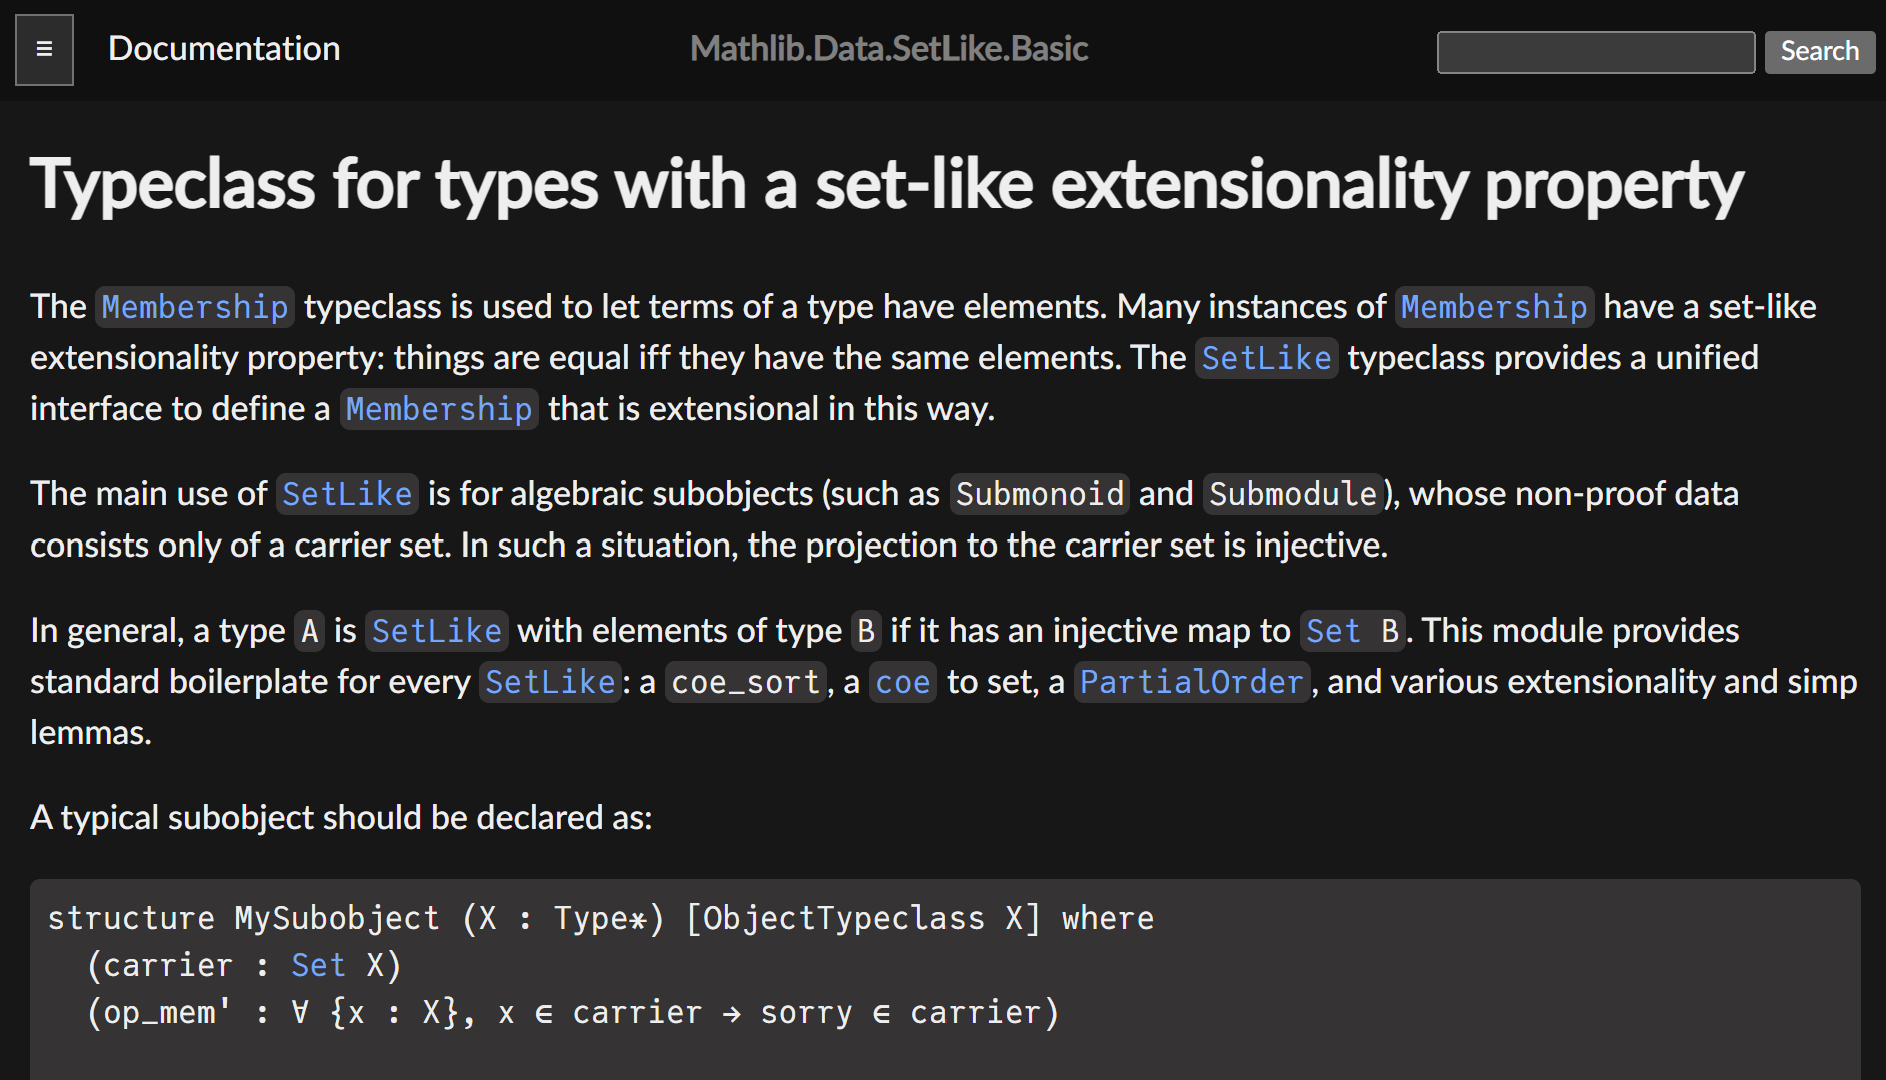
\includegraphics[width=\textwidth]{SetLikeDocs}
\end{frame}

\begin{frame}[fragile]
\frametitle{What I actually did}
\begin{lstlisting}[basicstyle=\ttfamily\footnotesize]
class Subcomplex (C D : Set X) [RelCWComplex C D] (E : Set X) where
  I : Π n, Set (cell C D n)
  closed : IsClosed E
  union : 
    D ∪ ⋃ (n : ℕ) (j : I n), openCell (C := C) (D := D) n j = E
\end{lstlisting}
\end{frame}

\begin{frame}[fragile]
\framtitle{The problem}
\begin{lstlisting}
instance CWComplex.instEmpty : CWComplex (∅ : Set X) := ... 


\end{lstlisting}
\end{frame}

\end{document}